% Options for packages loaded elsewhere
\PassOptionsToPackage{unicode}{hyperref}
\PassOptionsToPackage{hyphens}{url}
\documentclass[
]{article}
\usepackage{xcolor}
\usepackage{amsmath,amssymb}
\setcounter{secnumdepth}{-\maxdimen} % remove section numbering
\usepackage{iftex}
\ifPDFTeX
  \usepackage[T1]{fontenc}
  \usepackage[utf8]{inputenc}
  \usepackage{textcomp} % provide euro and other symbols
\else % if luatex or xetex
  \usepackage{unicode-math} % this also loads fontspec
  \defaultfontfeatures{Scale=MatchLowercase}
  \defaultfontfeatures[\rmfamily]{Ligatures=TeX,Scale=1}
\fi
\usepackage{lmodern}
\ifPDFTeX\else
  % xetex/luatex font selection
\fi
% Use upquote if available, for straight quotes in verbatim environments
\IfFileExists{upquote.sty}{\usepackage{upquote}}{}
\IfFileExists{microtype.sty}{% use microtype if available
  \usepackage[]{microtype}
  \UseMicrotypeSet[protrusion]{basicmath} % disable protrusion for tt fonts
}{}
\makeatletter
\@ifundefined{KOMAClassName}{% if non-KOMA class
  \IfFileExists{parskip.sty}{%
    \usepackage{parskip}
  }{% else
    \setlength{\parindent}{0pt}
    \setlength{\parskip}{6pt plus 2pt minus 1pt}}
}{% if KOMA class
  \KOMAoptions{parskip=half}}
\makeatother
\usepackage{graphicx}
\makeatletter
\newsavebox\pandoc@box
\newcommand*\pandocbounded[1]{% scales image to fit in text height/width
  \sbox\pandoc@box{#1}%
  \Gscale@div\@tempa{\textheight}{\dimexpr\ht\pandoc@box+\dp\pandoc@box\relax}%
  \Gscale@div\@tempb{\linewidth}{\wd\pandoc@box}%
  \ifdim\@tempb\p@<\@tempa\p@\let\@tempa\@tempb\fi% select the smaller of both
  \ifdim\@tempa\p@<\p@\scalebox{\@tempa}{\usebox\pandoc@box}%
  \else\usebox{\pandoc@box}%
  \fi%
}
% Set default figure placement to htbp
\def\fps@figure{htbp}
\makeatother
% definitions for citeproc citations
\NewDocumentCommand\citeproctext{}{}
\NewDocumentCommand\citeproc{mm}{%
  \begingroup\def\citeproctext{#2}\cite{#1}\endgroup}
\makeatletter
 % allow citations to break across lines
 \let\@cite@ofmt\@firstofone
 % avoid brackets around text for \cite:
 \def\@biblabel#1{}
 \def\@cite#1#2{{#1\if@tempswa , #2\fi}}
\makeatother
\newlength{\cslhangindent}
\setlength{\cslhangindent}{1.5em}
\newlength{\csllabelwidth}
\setlength{\csllabelwidth}{3em}
\newenvironment{CSLReferences}[2] % #1 hanging-indent, #2 entry-spacing
 {\begin{list}{}{%
  \setlength{\itemindent}{0pt}
  \setlength{\leftmargin}{0pt}
  \setlength{\parsep}{0pt}
  % turn on hanging indent if param 1 is 1
  \ifodd #1
   \setlength{\leftmargin}{\cslhangindent}
   \setlength{\itemindent}{-1\cslhangindent}
  \fi
  % set entry spacing
  \setlength{\itemsep}{#2\baselineskip}}}
 {\end{list}}
\usepackage{calc}
\newcommand{\CSLBlock}[1]{\hfill\break\parbox[t]{\linewidth}{\strut\ignorespaces#1\strut}}
\newcommand{\CSLLeftMargin}[1]{\parbox[t]{\csllabelwidth}{\strut#1\strut}}
\newcommand{\CSLRightInline}[1]{\parbox[t]{\linewidth - \csllabelwidth}{\strut#1\strut}}
\newcommand{\CSLIndent}[1]{\hspace{\cslhangindent}#1}
\setlength{\emergencystretch}{3em} % prevent overfull lines
\providecommand{\tightlist}{%
  \setlength{\itemsep}{0pt}\setlength{\parskip}{0pt}}
\usepackage{bookmark}
\IfFileExists{xurl.sty}{\usepackage{xurl}}{} % add URL line breaks if available
\urlstyle{same}
\hypersetup{
  pdftitle={TRANSFORMANDO APIS EM INTERFACES CONVERSACIONAIS: VALIDAÇÃO DA ABORDAGEM OPENAPI-MCP PARA AGENTES BASEADOS EM IA},
  hidelinks,
  pdfcreator={LaTeX via pandoc}}

\title{\textbf{TRANSFORMANDO APIS EM INTERFACES CONVERSACIONAIS:
VALIDAÇÃO DA ABORDAGEM OPENAPI-MCP PARA AGENTES BASEADOS EM IA}}
\author{}
\date{}

\begin{document}
\maketitle

\subsubsection{Artigo em produção - Checklist de
produção}\label{artigo-em-produuxe7uxe3o---checklist-de-produuxe7uxe3o}

\begin{itemize}
\tightlist
\item[$\square$]
  Edição do artigo

  \begin{itemize}
  \tightlist
  \item[$\square$]
    Aplicar formatação da SATC

    \begin{itemize}
    \tightlist
    \item[$\square$]
      Definir o template do .docx com o Word
    \end{itemize}
  \item[$\boxtimes$]
    Referências

    \begin{itemize}
    \tightlist
    \item[$\boxtimes$]
      Formatação ABNT
    \end{itemize}
  \end{itemize}
\item[$\square$]
  Escrita

  \begin{itemize}
  \tightlist
  \item[$\boxtimes$]
    Resumo
  \item[$\boxtimes$]
    Introdução
  \item[$\boxtimes$]
    Material e métodos
  \item[$\boxtimes$]
    Revisão e entrega parcial (nota 4.5/5)
  \item[$\square$]
    Desenvolvimento
  \item[$\square$]
    Resultados e discussão
  \item[$\square$]
    Considerações finais
  \item[$\square$]
    Revisão após finalizar o artigo
  \end{itemize}
\end{itemize}

\textbf{Lucas de Castro Zanoni}\footnote{Graduando em Engenharia de
  software no semestre letivo de 2025-1. E-mail:
  castro.lucas290@gmail.com}

\textbf{Thyerri Fernandes Mezzari}\footnote{Professor do Centro
  Universitário UniSATC E-mail: thyerri.mezzari@satc.edu.br}

Resumo: Este trabalho apresenta um estudo experimental de integração de
agentes conversacionais baseados em inteligência artificial a soluções
web através da especificação OpenAPI combinada com o protocolo Model
Context Protocol (MCP). A pesquisa investiga como especificações OpenAPI
podem ser automaticamente convertidas em servidores MCP, permitindo que
modelos de linguagem de grande escala (LLMs) interajam de forma
padronizada e segura com sistemas externos. Para garantir uma análise
rigorosa e reprodutível, foi desenvolvida uma interface padronizada e
definidos critérios objetivos, fundamentando-se em referências
acadêmicas, guias de segurança, relatórios de mercado e documentações
oficiais de provedores de modelos de linguagem. O estudo envolveu a
implementação de uma prova de conceito que inclui um gerador automático
de servidores MCP a partir de especificações OpenAPI, um cliente de chat
capaz de gerenciar múltiplos servidores MCP simultaneamente, e
aplicações de teste para validação da abordagem. Foram aplicados testes
automatizados end-to-end, com ênfase em métricas de robustez, segurança
(incluindo red teaming e injeção de prompts) e usabilidade. Os
resultados demonstram a viabilidade e eficácia da integração
OpenAPI-MCP, fornecendo uma análise fundamentada sobre os benefícios,
desafios e limitações desta abordagem para a integração de agentes
conversacionais em sistemas complexos, promovendo acessibilidade,
usabilidade e confiabilidade.

\textbf{Palavras-chave:} agente conversacional, integração de sistemas,
inteligência artificial, OpenAPI, Model Context Protocol, segurança,
usabilidade.

\section{1 INTRODUÇÃO}\label{introduuxe7uxe3o}

A evolução das interfaces de usuário tem gerado uma diversidade de
padrões de design e usabilidade, resultando frequentemente em barreiras
para a plena acessibilidade e interação dos usuários com os sistemas
digitais. Com o aumento da complexidade do frontend e a multiplicidade
de paradigmas de interação, muitos usuários enfrentam dificuldades
significativas para utilizar efetivamente as funcionalidades oferecidas
pelas soluções web modernas (RAPP et al., 2018) (KOCABALLI et al.,
2019). Nesse contexto, a ascensão dos Modelos de Linguagem de Grande
Escala (LLMs), como os desenvolvidos por OpenAI, Anthropic e Google, tem
impulsionado o desenvolvimento de agentes conversacionais mais avançados
e adaptáveis (ANTHROPIC, 2024a; OPENAI, 2022). Nos últimos anos, avanços
em modelos baseados em Transformer, como o BERT (2018), que aprimorou a
compreensão textual, e o GPT-3 (2020), que ampliou as capacidades
generativas e o aprendizado com poucos exemplos (\emph{few-shot}),
permitiram que os LLMs realizassem tarefas cada vez mais complexas a
partir de simples instruções em linguagem natural. Esses avanços
consolidaram os LLMs como interfaces conversacionais robustas e eficazes
para integração com sistemas.

Diante desse cenário, estudos recentes têm demonstrado que agentes
conversacionais podem aprimorar significativamente a experiência do
usuário ao simplificar interações com sistemas complexos (FAST et al.,
2017). Além disso, a implementação de interfaces baseadas em linguagem
natural tem mostrado potencial para melhorar a usabilidade em contextos
domésticos e inteligentes, reduzindo o tempo e o esforço necessários
para completar tarefas complexas (GUO et al., 2024). Ademais, tais
interfaces oferecem vantagens consideráveis em termos de acessibilidade,
permitindo uma comunicação mais inclusiva e adaptável a usuários com
diferentes necessidades especiais (LISTER et al., 2020) (DENG, 2023).
Para que esses benefícios sejam efetivamente alcançados em soluções web,
é fundamental avaliar as diferentes estratégias de integração desses
agentes aos sistemas existentes.

Nesse sentido, este estudo aborda experimentalmente a integração de
agentes conversacionais baseados em IA a sistemas web através da
especificação OpenAPI combinada com o protocolo emergente MCP (Model
Context Protocol). Esta abordagem permite que especificações OpenAPI
sejam automaticamente convertidas em servidores MCP, criando uma ponte
padronizada entre modelos de linguagem e sistemas externos. A solução
será avaliada quanto a desempenho, segurança, facilidade de
implementação e experiência do usuário, com foco específico na
capacidade de gerenciar múltiplos servidores MCP simultaneamente e na
eficácia da geração automática de código.

Dessa forma, a problemática central desta pesquisa reside na questão:
como a combinação da especificação OpenAPI com o protocolo MCP pode
facilitar a integração eficiente e segura de agentes conversacionais
baseados em IA com sistemas web existentes? Essa pergunta reflete a
necessidade crescente de soluções padronizadas que democratizem o acesso
à tecnologia, reduzindo a complexidade de integração e tornando sistemas
especializados mais acessíveis através de interfaces conversacionais
naturais.

A relevância deste estudo evidencia-se pelo potencial transformador que
os agentes conversacionais representam para a área de interação
humano-computador. Ao implementar um sistema intermediário capaz de
interpretar linguagem natural e traduzi-la em ações específicas dentro
de um sistema, cria-se uma ponte que permite aos usuários interagir de
forma mais intuitiva e natural com as tecnologias digitais. Esta
abordagem tem o potencial de mitigar as barreiras impostas por
interfaces complexas, contribuindo para uma maior inclusão digital e
para a melhoria da experiência do usuário em diversos contextos de
aplicação.

\section{2 PROCEDIMENTO EXPERIMENTAL}\label{procedimento-experimental}

Este estudo adota uma abordagem experimental estruturada em etapas
sequenciais para investigar a viabilidade e eficácia da integração de
agentes conversacionais baseados em IA a sistemas web através da
especificação OpenAPI combinada com o protocolo Model Context Protocol
(MCP). A pesquisa será examinada com base em uma prova de conceito
prática, desenvolvida para validar sua viabilidade técnica e avaliar
objetivamente aspectos funcionais e não-funcionais da solução proposta.

Inicialmente, será conduzida uma revisão sistemática da literatura,
consolidando conhecimentos científicos sobre integração OpenAPI-MCP e
embasando teoricamente a fase experimental. Na sequência, a estratégia
será implementada e testada por meio de uma prova de conceito
abrangente, incluindo o desenvolvimento de um gerador automático de
servidores MCP, um cliente de chat para gerenciamento de múltiplos
servidores, e aplicações de teste para validação da abordagem.

Os critérios de avaliação definidos incluem desempenho, segurança,
facilidade de implementação, manutenibilidade e experiência do usuário.
Para assegurar resultados objetivos e reproduzíveis, os testes incluirão
análises automatizadas end-to-end, medidas de robustez e segurança (como
testes de red teaming e proteção contra injeção de prompts) e avaliações
qualitativas de usabilidade. Os resultados serão sistematicamente
documentados e analisados, permitindo identificar desafios, vantagens e
limitações intrínsecas à integração OpenAPI-MCP e demonstrando sua
aplicabilidade prática para diferentes contextos de uso.

\subsection{2.1 MATERIAIS}\label{materiais}

Para garantir a rigorosidade científica e a reprodutibilidade dos
experimentos conduzidos neste estudo, é essencial uma seleção criteriosa
dos materiais e ferramentas utilizados. Esta seção detalha os recursos
específicos empregados na condução desta pesquisa, justificando sua
escolha baseada na eficiência, popularidade, robustez e aplicabilidade
prática dentro do contexto dos agentes conversacionais e integração de
sistemas.

\subsubsection{2.1.1 NODE.JS PARA DESENVOLVIMENTO DAS PROVAS DE
CONCEITO}\label{node.js-para-desenvolvimento-das-provas-de-conceito}

Node.js foi escolhido como plataforma principal para o desenvolvimento
das provas de conceito devido à sua comprovada eficácia na integração de
sistemas baseados em inteligência artificial (IA), especialmente com
agentes conversacionais e LLMs. A plataforma é amplamente adotada devido
à sua arquitetura orientada a eventos e capacidade de gerenciar
eficientemente múltiplas conexões simultâneas, essencial para aplicações
que exigem respostas rápidas em tempo real (CHEREDNICHENKO et al.,
2024).

Relatórios da \emph{Red Hat} destacam que o uso eficiente da arquitetura
assíncrona do Node.js possibilita a criação de agentes baseados em LLMs
com alta performance e escalabilidade. Isso garante um gerenciamento
eficiente de múltiplas operações paralelas, essencial para aplicações
intensivas em IA e integração com APIs externas (BLOG, 2024).

\subsubsection{\texorpdfstring{2.1.2 TESTES \emph{END-TO-END}
(E2E)}{2.1.2 TESTES END-TO-END (E2E)}}\label{testes-end-to-end-e2e}

O \emph{Framework} de Gerenciamento de Riscos de IA do NIST (OPREA;
VASSILEV, 2023) destaca a importância de avaliar o desempenho de
sistemas de IA de forma abrangente, defendendo que testes de integração
devem avaliar os sistemas de ponta a ponta para identificar erros de
integração e garantir a precisão das respostas em cenários realistas.
Testes rigorosos como esses não apenas identificam problemas de
integração, mas também asseguram às partes interessadas que o sistema se
comporta conforme o esperado em condições do mundo real.

A injeção de \emph{prompt} representa um risco significativo em
implantações de LLMs em nosso cenário, no qual o modelo possui acesso a
dados e sistemas potencialmente críticos, incluindo, ocasionalmente,
conexões diretas com dados brutos de banco de dados. O guia de riscos da
OWASP (JOHN et al., 2025) classifica a injeção de \emph{prompt} como uma
ameaça crítica à segurança, destacando a necessidade de procedimentos de
teste rigorosos para garantir que agentes conversacionais baseados em
LLMs não revelem inadvertidamente dados sensíveis ou contornem
restrições do sistema quando expostos a entradas maliciosas.
Recentemente, Wu et al.~(2023) (WU et al., 2023) demonstraram que
ataques de \emph{jailbreak} --- um tipo avançado de injeção de
\emph{prompt} --- podem burlar as salvaguardas éticas de modelos como o
ChatGPT em até 67\% dos casos, gerando conteúdos prejudiciais como
extorsão e desinformação.

Com isso em mente, o uso de testes E2E pode ser utilizado para avaliar a
resiliência da implementação ao simular entradas adversárias, processo
conhecido como \emph{red teaming}. Segundo Inie et al.~(2025) (INIE;
STRAY; DERCZYNSKI, 2025), o \emph{red teaming} desafia sistematicamente
sistemas de IA com \emph{prompts} adversários projetados para testar
seus limites e mecanismos de segurança. Ao encapsular consultas do
usuário com lembretes de responsabilidade ética (e.g., ``Você deve ser
um ChatGPT responsável''), o método reduziu a taxa de sucesso de
\emph{jailbreaks} para 19\%, mantendo a funcionalidade padrão do modelo
--- um resultado validado através de testes E2E em 540 cenários
adversarialmente projetados (WU et al., 2023).

\subsubsection{2.1.3 MODELOS DE LINGUAGEM DE GRANDE ESCALA
(LLMs)}\label{modelos-de-linguagem-de-grande-escala-llms}

Os LLMs, incluindo tecnologias como OpenAI GPT, Anthropic e modelos
disponibilizados pela Google, são essenciais neste estudo devido à sua
capacidade de interpretar e gerar linguagem natural de forma avançada e
eficaz. Estes modelos foram selecionados por sua performance comprovada
e ampla adoção em pesquisas acadêmicas e no mercado corporativo,
proporcionando um sólido embasamento para as funcionalidades de
interação do agente conversacional.

\paragraph{2.1.3.1 HISTÓRICO DO DESENVOLVIMENTO DE LLMS
(2018--2023)}\label{histuxf3rico-do-desenvolvimento-de-llms-20182023}

Nos últimos cinco anos, os LLMs evoluíram rapidamente, a partir da
arquitetura Transformer. O lançamento do BERT (2018) mostrou avanços em
compreensão textual, enquanto a série GPT demonstrou fortes capacidades
generativas. O GPT-3 (2020), com 175 bilhões de parâmetros, evidenciou
habilidades emergentes de aprendizado com poucos exemplos
(\emph{few-shot}), ampliando o escopo de tarefas possíveis por meio de
simples instruções em linguagem natural (BROWN et al., 2020).

A partir de 2022, o foco da pesquisa passou a ser o aprimoramento do
raciocínio e alinhamento dos LLMs. Técnicas como \emph{Chain-of-Thought
prompting} permitiram que os modelos resolvessem problemas complexos de
forma mais eficaz (WEI et al., 2023). O uso de Reinforcement Learning
from Human Feedback (RLHF), como nos modelos InstructGPT e
posteriormente ChatGPT, melhorou a capacidade dos LLMs de seguir
instruções com mais segurança e consistência. Esses avanços
estabeleceram as bases para o uso dos LLMs como interfaces
conversacionais robustas em cenários de integração com sistemas (OPENAI,
2022).

\paragraph{2.1.3.2 EXTENSÃO DE JANELA DE
CONTEXTO}\label{extensuxe3o-de-janela-de-contexto}

Com o avanço dos modelos, observou-se uma tendência significativa no
aumento das janelas de contexto --- a quantidade de tokens que um LLM
pode processar em uma única interação. Modelos como o Claude 3 já
alcançam até 100.000 tokens (ANTHROPIC, 2024b), enquanto versões
estendidas do GPT-4 suportam até 32.000 tokens (OPENAI, 2023a). Esse
aumento permite que os modelos processem documentos extensos, múltiplas
conversas ou grandes volumes de dados em uma única solicitação,
superando, em muitos casos, abordagens tradicionais baseadas em
retrieval-augmented generation (RAG), especialmente em tarefas que
exigem síntese contextual profunda.

A capacidade de manter longos contextos é altamente benéfica para
integração com sistemas -- um LLM pode manter diálogos prolongados,
lembrar estados extensos ou ingerir bancos de dados e logs inteiros de
uma só vez. No entanto, isso traz custos computacionais consideráveis, e
há esforços contínuos para utilizar essas janelas maiores de forma
eficiente (por exemplo, condensando ou focando a atenção nas partes mais
relevantes) (ANTHROPIC, 2024b; OPENAI, 2023a).

\paragraph{2.1.3.3 RACIOCÍNIO APRIMORADO E COMPREENSÃO PROFUNDA (DEEP
THINKING)}\label{raciocuxednio-aprimorado-e-compreensuxe3o-profunda-deep-thinking}

Os LLMs mais recentes apresentam avanços significativos em raciocínio,
planejamento e resolução de tarefas complexas. Técnicas como o
\emph{Chain-of-Thought prompting}, que induz os modelos a pensar em
etapas intermediárias, mostraram ganhos substanciais em tarefas que
exigem múltiplos passos lógicos (WEI et al., 2023). Além disso,
abordagens como \emph{tree-of-thought} e \emph{self-reflection} permitem
que os modelos reavaliem suas respostas e melhorem sua própria
performance iterativamente. Esses avanços tornam os LLMs mais confiáveis
para tarefas que exigem raciocínio profundo e tomada de decisão
estruturada, fundamentais para integração com sistemas complexos (YAO et
al., 2023).

\paragraph{2.1.3.4 USO DE FERRAMENTAS EM TEMPO REAL E INTERAÇÃO COM
SISTEMAS}\label{uso-de-ferramentas-em-tempo-real-e-interauxe7uxe3o-com-sistemas}

O avanço dos LLMs em ambientes de produção foi impulsionado por recursos
como o \emph{function calling} da OpenAI. Essa funcionalidade permite
que os modelos interpretem solicitações em linguagem natural e as
convertam em chamadas de funções estruturadas, conforme definido pelo
desenvolvedor. Por exemplo, ao receber uma instrução como ``agende uma
reunião para amanhã às 14h'', o modelo pode gerar uma chamada de função
com os parâmetros apropriados para interagir com uma API de calendário,
sem depender de engenharia de \emph{prompt} ou extração de texto
(OPENAI, 2023b). Essa abordagem, melhora significativamente a
confiabilidade em cenários de integração, permitindo que o modelo
obtenha dados estruturados de bancos de dados, chame APIs de negócios,
envie e-mails, entre outras ações, em vez de apenas tentar adivinhar a
resposta (OPENAI, 2023b).

Complementando essa capacidade, o \emph{Model Context Protocol} (MCP),
desenvolvido pela Anthropic (ANTHROPIC, 2024a; MODEL CONTEXT PROTOCOL
TEAM, 2025), oferece um padrão aberto para conectar LLMs a diversas
fontes de dados e ferramentas. O MCP estabelece uma arquitetura
cliente-servidor onde os modelos (clientes) podem acessar servidores MCP
que expõem recursos, \emph{prompts} e ferramentas de forma padronizada.
Isso elimina a necessidade de integrações personalizadas para cada fonte
de dados, promovendo uma interoperabilidade mais ampla e sustentável.

\subsubsection{2.1.4 FERRAMENTAS ESPECÍFICAS DE
INTEGRAÇÃO}\label{ferramentas-especuxedficas-de-integrauxe7uxe3o}

A pesquisa utiliza ferramentas específicas para a integração dos agentes
conversacionais com soluções \emph{web} através da abordagem
OpenAPI-MCP:

\begin{itemize}
\tightlist
\item
  \textbf{OpenAPI para Definição de Contratos de API:} foi selecionado
  devido à sua ampla adoção como padrão da indústria para definição de
  interfaces \emph{RESTful}, sendo reconhecido por facilitar a
  documentação consistente e interoperabilidade entre sistemas. Sua
  especificação permite descrever de maneira clara e estruturada os
  contratos das APIs, incluindo esquemas de autenticação como OAuth e
  chaves de API, essenciais para declarar uniformemente os requisitos de
  segurança das interfaces dos agentes conversacionais (OPENAPI
  INITIATIVE, 2023; THE POSTMAN TEAM, 2023).
\end{itemize}

A relevância do OpenAPI para agentes baseados em LLM reside na
possibilidade de fornecer uma descrição estruturada das capacidades
disponíveis para o agente. Por meio de uma definição formal e
padronizada, os modelos de linguagem podem interpretar diretamente as
interfaces, compreendendo quais operações podem ser solicitadas e como
realizá-las com segurança e eficiência. Essa abordagem já é aplicada por
sistemas como os plugins do ChatGPT, demonstrando sua efetividade para
integração direta entre LLMs e APIs externas (OPENAI, 2023c).

\begin{itemize}
\tightlist
\item
  \textbf{Model Context Protocol (MCP):} é um padrão aberto emergente
  para integração entre agentes de IA e sistemas externos, com o
  objetivo de padronizar como modelos acessam dados, serviços e
  ferramentas. Ele fornece uma arquitetura clara baseada em clientes e
  servidores, permitindo que agentes conversem com fontes externas de
  forma segura, modular e escalável. Desde seu lançamento aberto, no
  final de novembro de 2024, o protocolo ganhou tração significativa com
  a criação de diversos servidores prontos para PostgreSQL, GitHub,
  Slack, entre outros, além de SDKs em múltiplas linguagens (ANTHROPIC,
  2024c; MODEL CONTEXT PROTOCOL CONTRIBUTORS, 2024).
\end{itemize}

A adoção crescente é impulsionada pela comunidade ativa, o que demonstra
o potencial do MCP como um padrão de integração para sistemas baseados
em LLMs. Sua proposta de `porta universal' para conectar agentes a
ferramentas oferece flexibilidade e segurança: características
fundamentais quando agentes com poder de raciocínio, como LLMs, precisam
acessar recursos sensíveis de forma controlada e auditável (ANTHROPIC,
2024c).

\begin{itemize}
\tightlist
\item
  \textbf{Gerador MCP-OpenAPI:} para viabilizar a integração automática
  entre especificações OpenAPI e servidores MCP, foi desenvolvido um
  gerador especializado baseado no projeto mcp-openapi-server. Esta
  ferramenta analisa especificações OpenAPI e gera automaticamente
  servidores MCP correspondentes, incluindo validação de schemas,
  mapeamento de tipos de dados e tratamento de erros. O gerador suporta
  múltiplas especificações simultaneamente e permite configuração
  personalizada de autenticação e permissões, facilitando a criação de
  pontes padronizadas entre LLMs e sistemas externos sem necessidade de
  desenvolvimento manual para cada integração.
\end{itemize}

\subsection{2.2 MÉTODOS}\label{muxe9todos}

Para assegurar a rigorosidade científica e garantir a reprodutibilidade
dos experimentos conduzidos neste estudo, foi desenvolvida uma interface
padrão comum para avaliar todas as abordagens de integração. Essa
padronização viabiliza uma comparação justa e objetiva entre as
implementações, minimizando variáveis relacionadas à interface que
poderiam interferir nos resultados finais.

\subsubsection{2.2.1 Interface Comum de
Usuário}\label{interface-comum-de-usuuxe1rio}

A interface comum consiste em uma aplicação \emph{web} simples de chat,
desenvolvida utilizando React.js e TypeScript. A interface foi projetada
de forma minimalista, visando uma experiência consistente e objetiva,
independentemente da abordagem de integração utilizada.

\begin{figure}
\centering
\pandocbounded{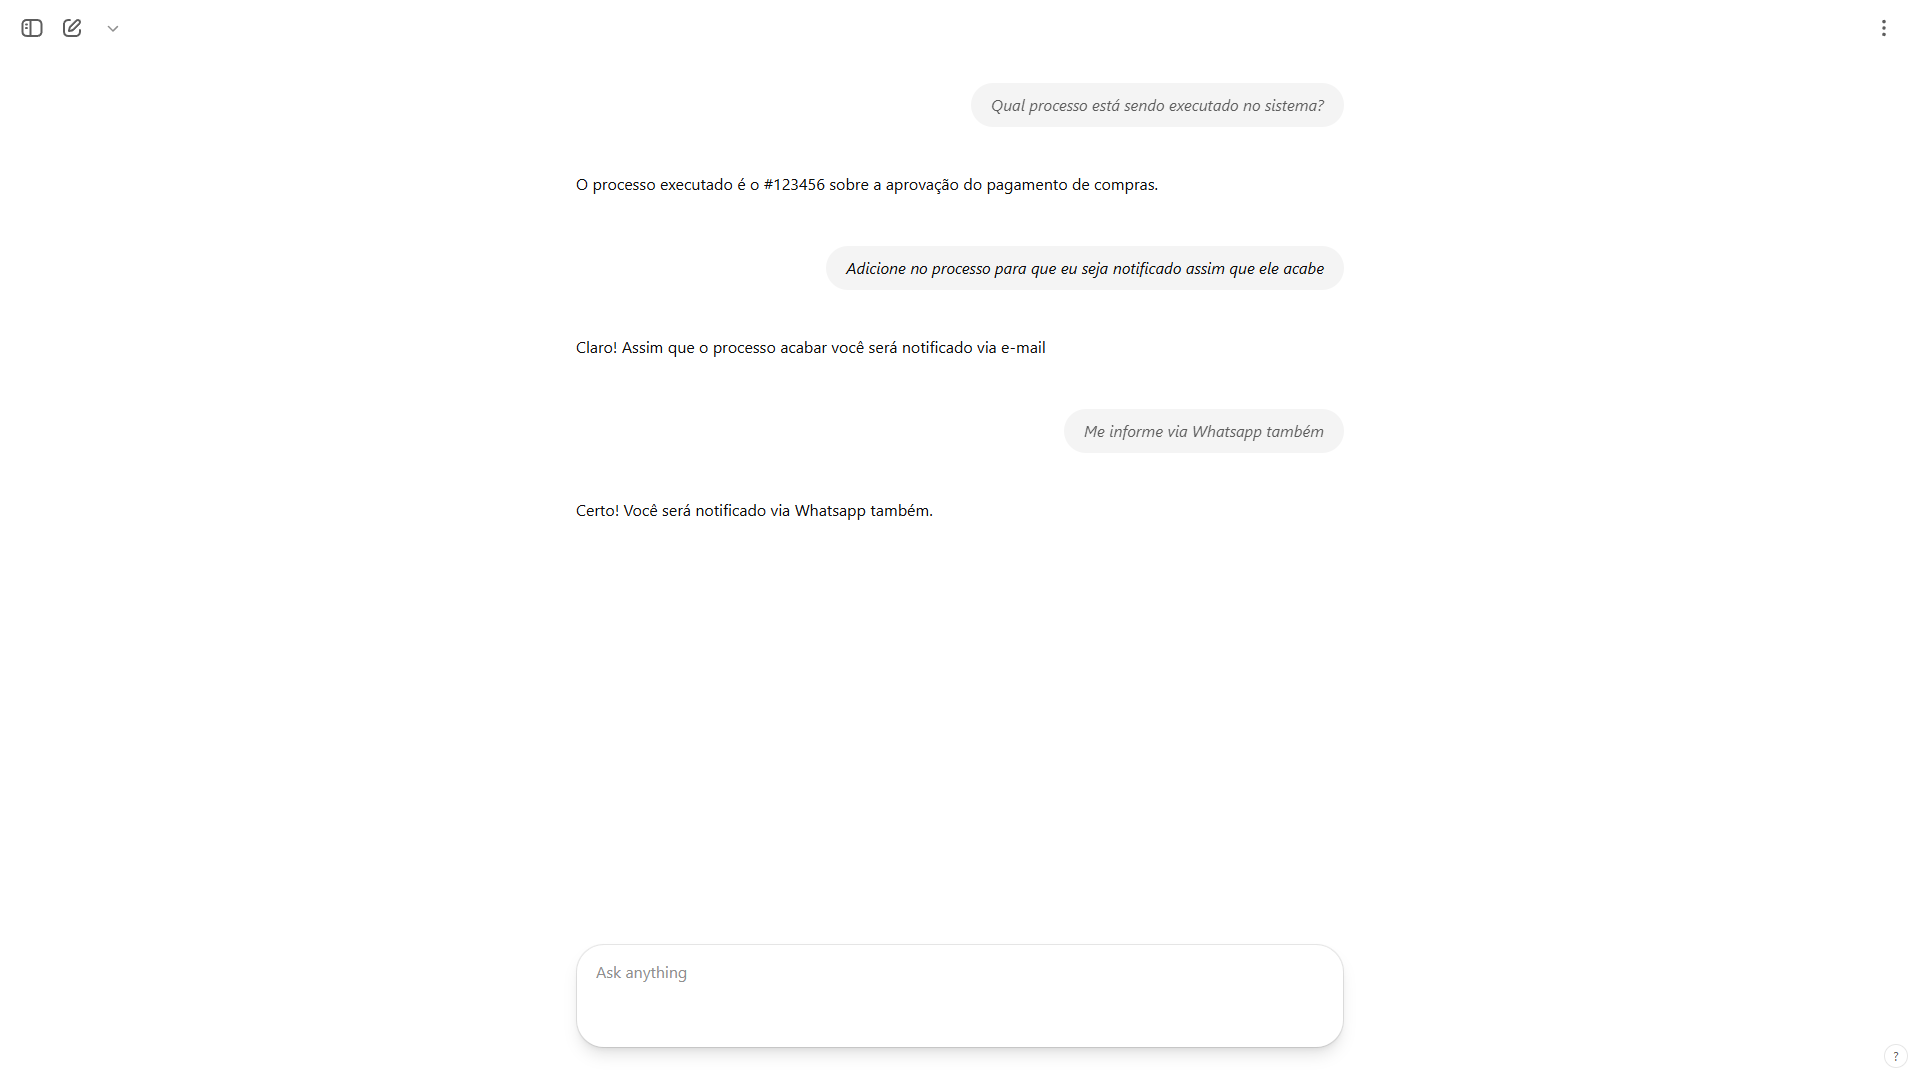
\includegraphics[keepaspectratio]{images/metodos/user-interface.jpg}}
\caption{Interface do Usuário}
\end{figure}

\paragraph{2.2.1.1 DESIGN DA INTERFACE}\label{design-da-interface}

A interface é composta por uma seção principal que exibe o histórico de
mensagens, onde as interações entre usuário e agente conversacional
aparecem de forma intercalada: as mensagens do agente são exibidas à
esquerda e as do usuário à direita, facilitando a distinção visual entre
os participantes da conversa. Abaixo do histórico, há um campo de
entrada de texto que permite ao usuário digitar e enviar novas
mensagens. Esse layout possibilita ao usuário acompanhar facilmente todo
o histórico da conversa e inserir novos \emph{prompts} de maneira
contínua e intuitiva.

\paragraph{2.2.1.2 Comunicação com
Backend}\label{comunicauxe7uxe3o-com-backend}

A comunicação entre frontend e backend será estabelecida por meio de uma
API REST síncrona, simplificando o processo de envio e retorno de
mensagens. Cada consulta feita pelo usuário gerará uma única requisição
ao backend que processará integralmente essa requisição utilizando um
LLM e devolverá uma resposta após concluir o processamento, mantendo o
fluxo de comunicação claro e previsível.

\subsubsection{2.2.2 Arquitetura e Fluxo de Integração do
Sistema}\label{arquitetura-e-fluxo-de-integrauxe7uxe3o-do-sistema}

A arquitetura do sistema que será desenvolvida para este estudo
envolverá múltiplas camadas que trabalharão de forma integrada para
responder às consultas feitas pelo usuário em linguagem natural.
Inicialmente, as consultas serão recebidas pela interface \emph{web} e
encaminhadas ao backend, onde o modelo de linguagem executará o processo
de análise e interpretação.

\begin{figure}
\centering
\pandocbounded{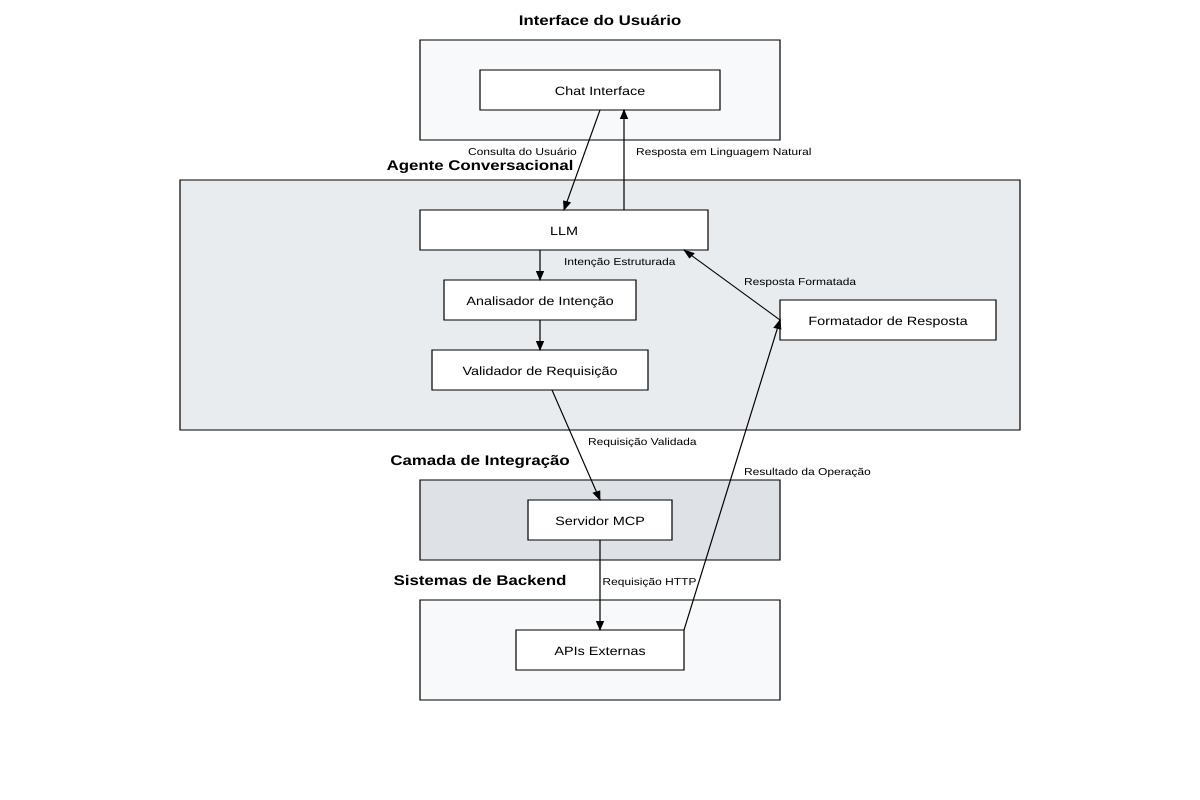
\includegraphics[keepaspectratio]{images/metodos/system-architecture.jpg}}
\caption{Arquitetura do Sistema}
\end{figure}

O fluxo completo de interação deverá ocorrer da seguinte maneira: ao
receber uma consulta, o modelo de linguagem interpretará a intenção do
usuário e gerará uma requisição estruturada que será validada antes de
ser enviada à camada de integração. Essa camada utilizará diferentes
abordagens (ORM, MCP ou conexão direta com o banco de dados) para
acessar sistemas backend, como modelos de dados, APIs externas ou bancos
de dados diretamente. Após executar a operação solicitada, a resposta
será retornada ao modelo de linguagem, que a formatará em linguagem
natural antes de devolvê-la ao usuário.

\begin{figure}
\centering
\pandocbounded{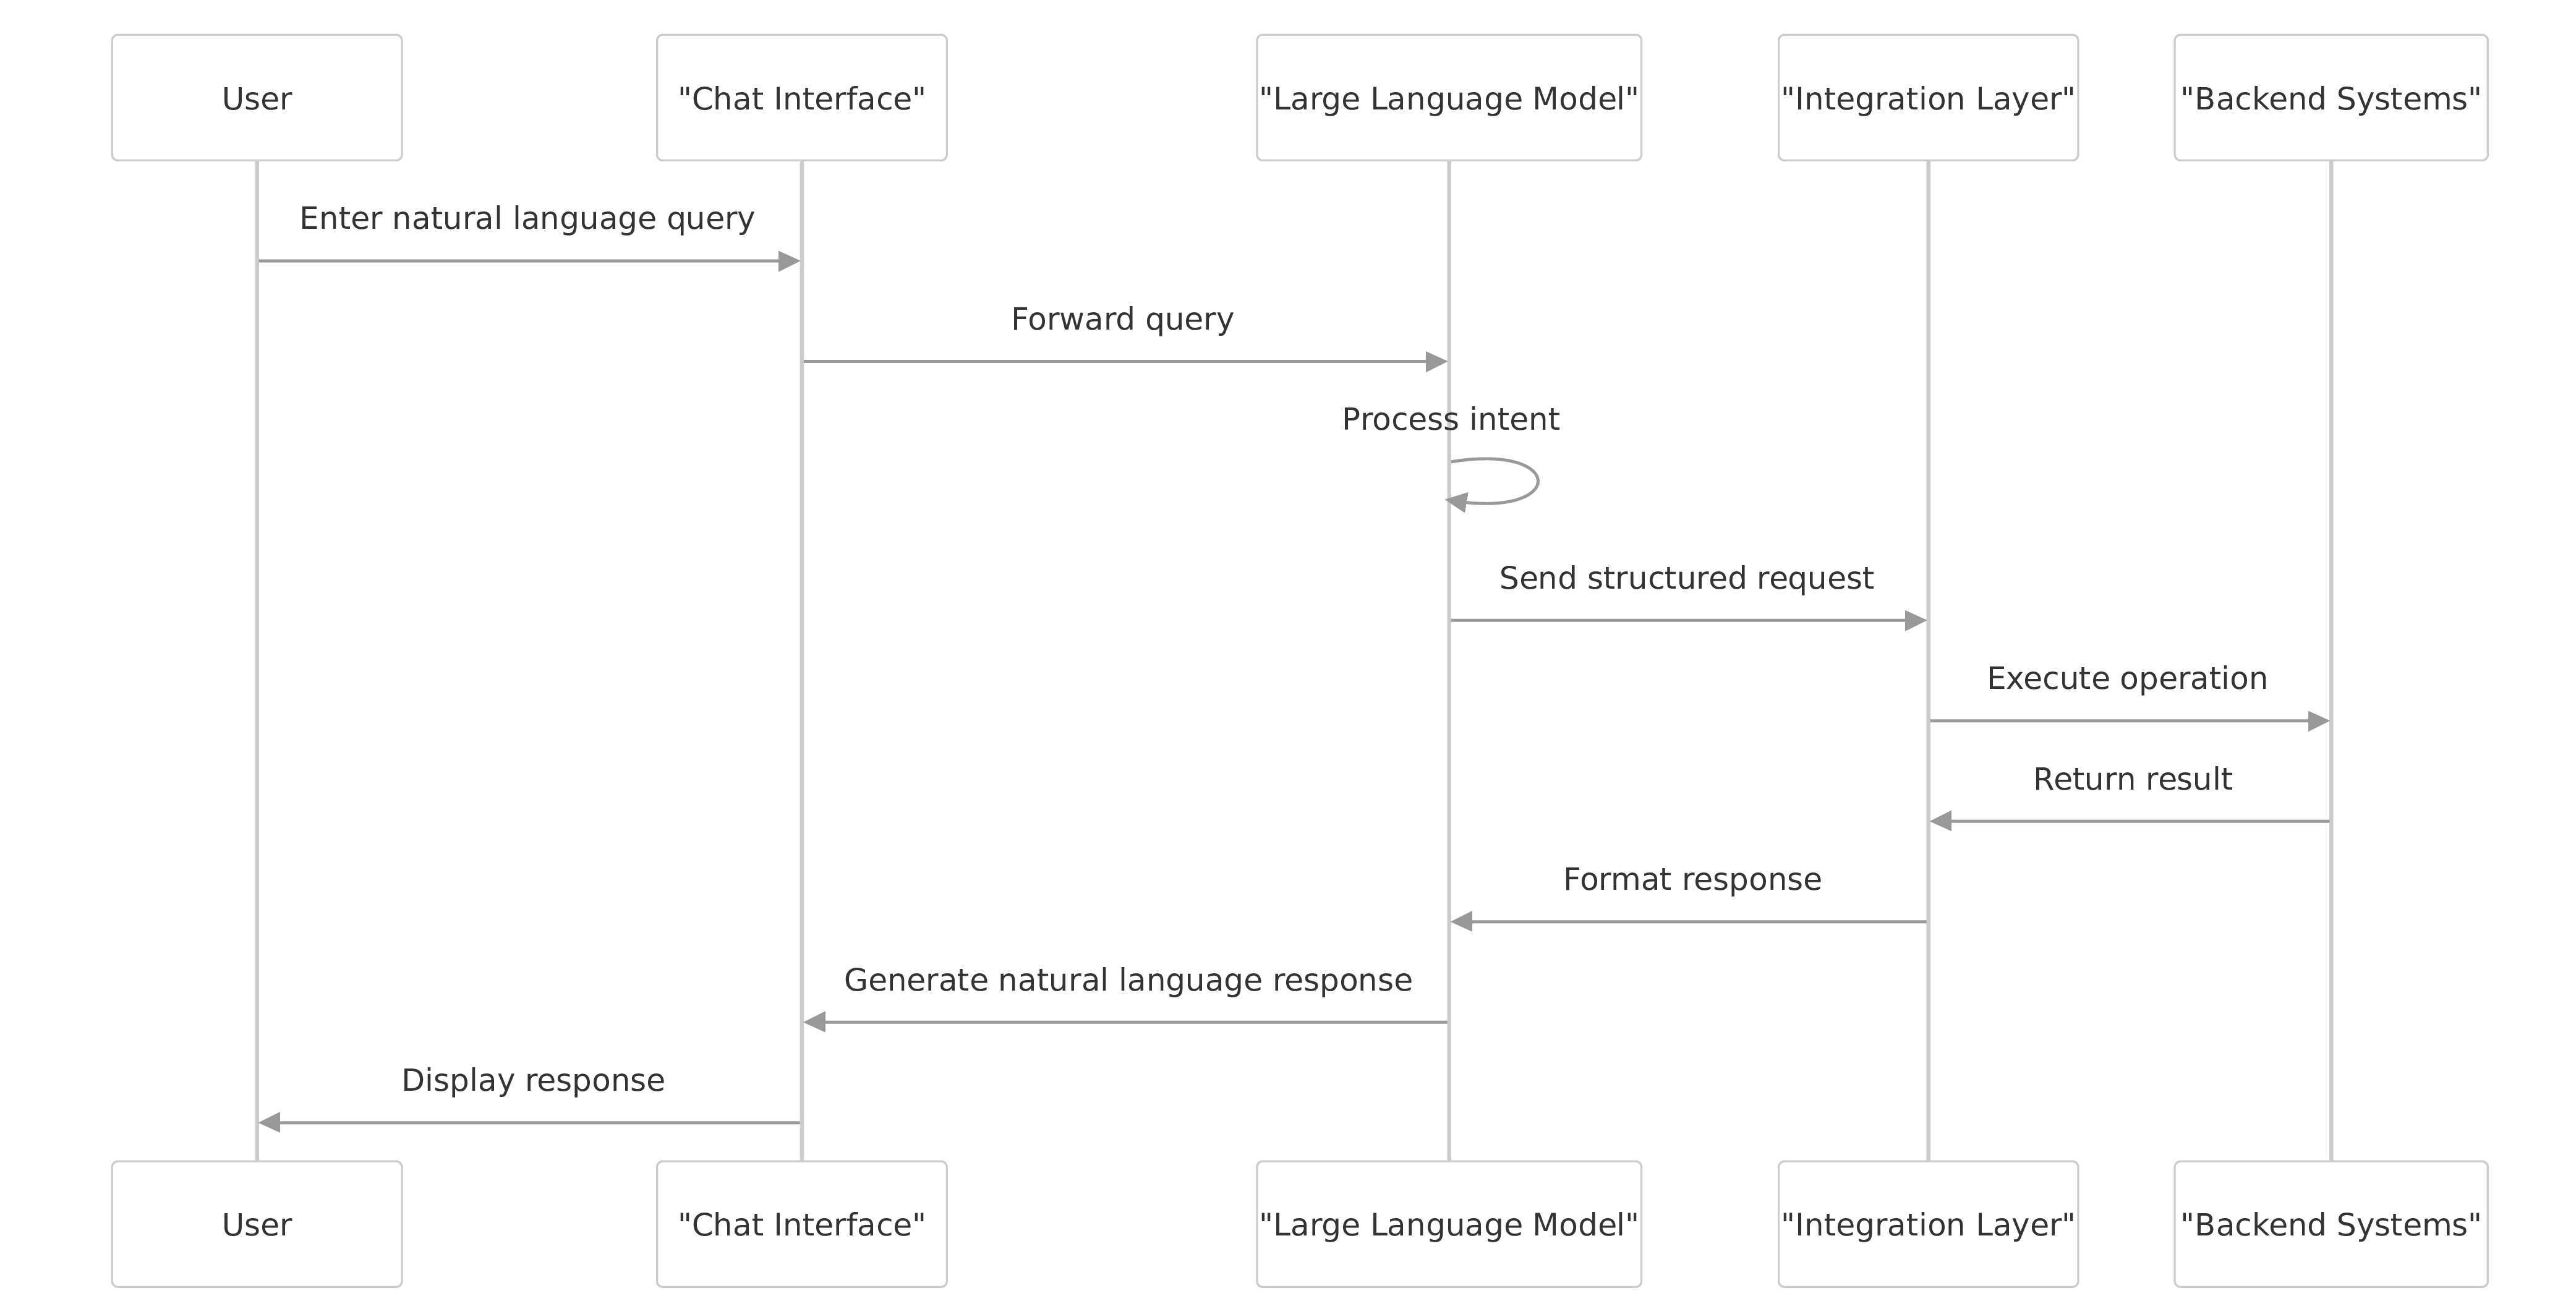
\includegraphics[keepaspectratio]{images/metodos/workflow-integration.jpg}}
\caption{Diagrama de Workflow do Agente}
\end{figure}

\subsubsection{2.2.3 Coleta de Métricas via Testes
E2E}\label{coleta-de-muxe9tricas-via-testes-e2e}

Testes End-to-End (E2E) são essenciais para avaliar não apenas o
desempenho e a segurança, mas também a experiência geral do usuário com
sistemas integrados a LLMs. Os testes são automatizados, executados
regularmente em ambiente controlado para assegurar resultados
consistentes e comparáveis.

Os testes envolvem: - Avaliação detalhada da performance, incluindo
tempos totais de resposta, tempo específico do processamento pelo modelo
de linguagem e latência da rede. - Análise da confiabilidade através da
taxa de sucesso das requisições e frequência de erros críticos e não
críticos. - Avaliação de segurança utilizando técnicas de \emph{Red
Team}, incluindo a tentativa sistemática de exploração de
vulnerabilidades com injeção de \emph{prompts} e validação dos controles
de acesso. - Mensuração da experiência do usuário, utilizando avaliações
qualitativas da clareza das respostas e pesquisas estruturadas de
satisfação com escalas Likert.

Os testes E2E são executados de forma automatizada em ambiente
controlado, simulando diferentes cenários de uso e condições de carga,
permitindo uma avaliação objetiva e reproduzível de cada abordagem de
integração.

Esta padronização da coleta de métricas via testes E2E garante que as
diferenças observadas entre as abordagens sejam resultado direto das
suas características de implementação, e não de variações na experiência
do usuário ou na forma de coleta de dados.

Em seguida, os testes são executados automaticamente, variando desde
consultas simples até cenários complexos e ataques adversários
simulados. As métricas obtidas são automaticamente registradas para
garantir uma coleta padronizada e confiável dos dados. Finalmente, uma
análise automatizada gera relatórios detalhados, permitindo uma
comparação objetiva e precisa entre as diferentes abordagens
implementadas.

\subsection{3. DESENVOLVIMENTO}\label{desenvolvimento}

A implementação da solução OpenAPI-MCP foi estruturada em quatro
componentes principais: um gerador automático de servidores MCP a partir
de especificações OpenAPI, um cliente de chat capaz de gerenciar
múltiplos servidores MCP simultaneamente, aplicações de teste para
validação da abordagem, e uma suíte de testes automatizados para
avaliação da solução. Esta seção detalha a arquitetura, implementação e
considerações técnicas de cada componente.

\subsubsection{3.1 Gerador Automático de Servidores MCP
(mcp-openapi-server)}\label{gerador-automuxe1tico-de-servidores-mcp-mcp-openapi-server}

O componente central da solução é um gerador automático que converte
especificações OpenAPI em servidores MCP funcionais. Esta ferramenta
elimina a necessidade de desenvolvimento manual de integrações
personalizadas para cada API, promovendo padronização e escalabilidade.

\paragraph{3.1.1 Arquitetura do Gerador}\label{arquitetura-do-gerador}

O gerador é implementado em TypeScript e Node.js, estruturado em três
camadas principais:

\begin{enumerate}
\def\labelenumi{\arabic{enumi}.}
\tightlist
\item
  \textbf{Camada de Análise OpenAPI}

  \begin{itemize}
  \tightlist
  \item
    Parser de especificações OpenAPI 3.0+
  \item
    Validação de schemas e estruturas
  \item
    Extração de metadados de endpoints e operações
  \end{itemize}
\item
  \textbf{Camada de Mapeamento MCP}

  \begin{itemize}
  \tightlist
  \item
    Conversão de operações OpenAPI para ferramentas MCP
  \item
    Mapeamento de tipos de dados entre especificações
  \item
    Geração de documentação automática
  \end{itemize}
\item
  \textbf{Camada de Geração de Código}

  \begin{itemize}
  \tightlist
  \item
    Geração de servidores MCP em TypeScript
  \item
    Implementação de validação de entrada
  \item
    Tratamento de erros e logging
  \end{itemize}
\end{enumerate}

\begin{figure}
\centering
\pandocbounded{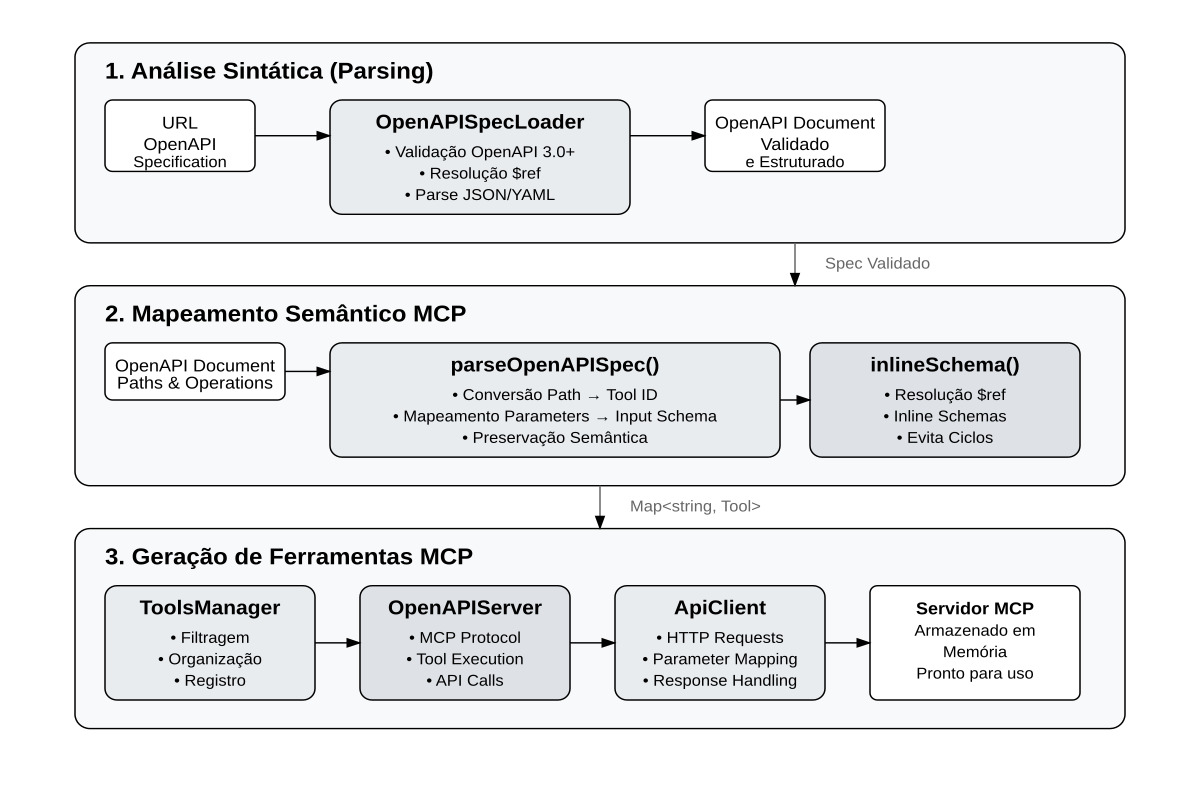
\includegraphics[keepaspectratio]{images/desenvolvimento/mcp-generator-architecture.jpg}}
\caption{Arquitetura do Gerador MCP-OpenAPI}
\end{figure}

\paragraph{3.1.2 Processo de Geração}\label{processo-de-gerauxe7uxe3o}

O processo de geração segue os seguintes passos:

\begin{enumerate}
\def\labelenumi{\arabic{enumi}.}
\item
  \textbf{Carregamento da Especificação:} O gerador carrega e valida
  arquivos OpenAPI em formato JSON ou YAML, verificando conformidade com
  a especificação OpenAPI 3.0+.
\item
  \textbf{Análise de Endpoints:} Cada endpoint é analisado para extrair
  informações sobre operações HTTP, parâmetros, schemas de entrada e
  saída, e requisitos de autenticação.
\item
  \textbf{Mapeamento para MCP:} As operações são convertidas em
  ferramentas MCP, com mapeamento automático de tipos de dados e geração
  de descrições baseadas na documentação OpenAPI.
\item
  \textbf{Geração do Servidor:} É gerado um servidor MCP completo em
  TypeScript, incluindo validação de entrada, tratamento de erros, e
  proxy para as APIs originais.
\end{enumerate}

\paragraph{3.1.3 Funcionalidades
Implementadas}\label{funcionalidades-implementadas}

\begin{itemize}
\tightlist
\item
  \textbf{Suporte a Múltiplas APIs:} Capacidade de gerar servidores para
  múltiplas especificações OpenAPI simultaneamente
\item
  \textbf{Validação Automática:} Validação de entrada baseada em schemas
  OpenAPI
\item
  \textbf{Tratamento de Autenticação:} Suporte a diferentes métodos de
  autenticação (API Key, Bearer Token, OAuth)
\item
  \textbf{Gestão de Erros:} Tratamento robusto de erros com mapeamento
  para códigos de status HTTP apropriados
\item
  \textbf{Logging e Monitoramento:} Sistema de logging integrado para
  auditoria e debugging
\end{itemize}

\subsubsection{3.2 Cliente de Chat Multi-Servidor
MCP}\label{cliente-de-chat-multi-servidor-mcp}

O cliente de chat foi desenvolvido para demonstrar e validar a
capacidade de gerenciar múltiplos servidores MCP simultaneamente,
permitindo que um único agente conversacional acesse diferentes sistemas
através de suas respectivas especificações OpenAPI.

\paragraph{3.2.1 Arquitetura do Cliente}\label{arquitetura-do-cliente}

A arquitetura do cliente é baseada em uma aplicação web com frontend em
HTML/JavaScript e backend em Node.js:

\begin{enumerate}
\def\labelenumi{\arabic{enumi}.}
\tightlist
\item
  \textbf{Frontend (chat.html)}

  \begin{itemize}
  \tightlist
  \item
    Interface de chat minimalista e responsiva
  \item
    Exibição de histórico de conversas
  \item
    Campo de entrada para comandos do usuário
  \item
    Indicadores visuais de status das operações
  \end{itemize}
\item
  \textbf{Backend (backend-server.js)}

  \begin{itemize}
  \tightlist
  \item
    Servidor Express.js para gerenciamento de requisições
  \item
    Cliente MCP para comunicação com múltiplos servidores
  \item
    Integração com LLMs via OpenAI API
  \item
    Gerenciamento de sessões e contexto de conversa
  \end{itemize}
\end{enumerate}

\begin{figure}
\centering
\pandocbounded{\includegraphics[keepaspectratio]{images/desenvolvimento/chat-client-architecture.jpg}}
\caption{Arquitetura do Cliente de Chat}
\end{figure}

\paragraph{3.2.2 Gerenciamento de Múltiplos Servidores
MCP}\label{gerenciamento-de-muxfaltiplos-servidores-mcp}

O cliente implementa um sistema sofisticado para gerenciar conexões
simultâneas com múltiplos servidores MCP:

\begin{itemize}
\tightlist
\item
  \textbf{Pool de Conexões:} Mantém conexões ativas com todos os
  servidores MCP configurados
\item
  \textbf{Descoberta de Ferramentas:} Automaticamente descobre e
  cataloga ferramentas disponíveis em cada servidor
\item
  \textbf{Roteamento Inteligente:} Determina qual servidor usar baseado
  na intenção do usuário e ferramentas disponíveis
\item
  \textbf{Agregação de Resultados:} Combina resultados de múltiplos
  servidores quando necessário
\end{itemize}

\paragraph{3.2.3 Integração com LLMs}\label{integrauxe7uxe3o-com-llms}

O sistema utiliza a API da OpenAI com funcionalidade de \emph{function
calling} para integração com os servidores MCP:

\begin{enumerate}
\def\labelenumi{\arabic{enumi}.}
\tightlist
\item
  \textbf{Conversão de Ferramentas:} Ferramentas MCP são automaticamente
  convertidas para o formato de funções da OpenAI
\item
  \textbf{Gestão de Contexto:} Mantém contexto de conversa incluindo
  histórico de chamadas de ferramentas
\item
  \textbf{Tratamento de Respostas:} Processa respostas de ferramentas e
  as integra na conversa natural
\end{enumerate}

\subsubsection{3.3 Aplicações de Teste}\label{aplicauxe7uxf5es-de-teste}

Para validar a eficácia da solução, foram desenvolvidas duas aplicações
de teste que expõem APIs RESTful com especificações OpenAPI:

\paragraph{3.3.1 Sistema de Gerenciamento de Equipamentos
(equipments-dummy-app)}\label{sistema-de-gerenciamento-de-equipamentos-equipments-dummy-app}

Esta aplicação simula um sistema de gerenciamento de equipamentos
industriais:

\begin{itemize}
\tightlist
\item
  \textbf{Operações CRUD:} Criação, leitura, atualização e exclusão de
  equipamentos
\item
  \textbf{Modelo de Dados:} Equipamentos com propriedades como nome,
  tipo, descrição e imagem
\item
  \textbf{API RESTful:} Endpoints padronizados seguindo convenções REST
\item
  \textbf{Especificação OpenAPI:} Documentação completa da API gerada
  automaticamente
\end{itemize}

\paragraph{3.3.2 Sistema de Gerenciamento de Profissionais
(professionals-dummy-app)}\label{sistema-de-gerenciamento-de-profissionais-professionals-dummy-app}

Esta aplicação simula um sistema de recursos humanos:

\begin{itemize}
\tightlist
\item
  \textbf{Gestão de Profissionais:} CRUD completo para dados de
  profissionais
\item
  \textbf{Hierarquia Organizacional:} Suporte a estruturas hierárquicas
  com níveis
\item
  \textbf{Biografia e Perfis:} Campos adicionais para informações
  detalhadas
\item
  \textbf{Integração com Equipamentos:} Relacionamento entre
  profissionais e equipamentos utilizados
\end{itemize}

\paragraph{3.3.3 Especificações
OpenAPI}\label{especificauxe7uxf5es-openapi}

Ambas as aplicações geram especificações OpenAPI completas que incluem:

\begin{itemize}
\tightlist
\item
  \textbf{Schemas de Dados:} Definições detalhadas de todos os modelos
  de dados
\item
  \textbf{Operações:} Documentação completa de todos os endpoints
  disponíveis
\item
  \textbf{Autenticação:} Especificação de métodos de autenticação
  suportados
\item
  \textbf{Exemplos:} Exemplos de requisições e respostas para cada
  operação
\end{itemize}

\subsubsection{3.4 Testes Automatizados e
Validação}\label{testes-automatizados-e-validauxe7uxe3o}

A solução inclui uma suíte abrangente de testes automatizados
implementados com Playwright para validação end-to-end:

\paragraph{3.4.1 Testes de
Funcionalidade}\label{testes-de-funcionalidade}

\begin{itemize}
\tightlist
\item
  \textbf{Operações CRUD:} Validação de todas as operações básicas
  através do chat
\item
  \textbf{Multi-servidor:} Testes de coordenação entre múltiplos
  servidores MCP
\item
  \textbf{Robustez:} Testes com entradas inválidas e cenários de erro
\end{itemize}

\paragraph{3.4.2 Testes de Segurança}\label{testes-de-seguranuxe7a}

\begin{itemize}
\tightlist
\item
  \textbf{Injeção de Prompt:} Tentativas sistemáticas de injeção
  maliciosa
\item
  \textbf{Validação de Entrada:} Verificação de sanitização adequada de
  dados
\item
  \textbf{Controle de Acesso:} Testes de autorização e autenticação
\end{itemize}

\paragraph{3.4.3 Testes de Performance}\label{testes-de-performance}

\begin{itemize}
\tightlist
\item
  \textbf{Latência:} Medição de tempos de resposta para diferentes tipos
  de operação
\item
  \textbf{Throughput:} Avaliação da capacidade de processamento
  simultâneo
\item
  \textbf{Uso de Recursos:} Monitoramento de consumo de memória e CPU
\end{itemize}

Esta implementação demonstra a viabilidade técnica da integração
OpenAPI-MCP, fornecendo uma base sólida para avaliação comparativa e
validação científica da abordagem proposta.

\section{4 RESULTADOS E DISCUSSÕES}\label{resultados-e-discussuxf5es}

A avaliação da solução OpenAPI-MCP foi conduzida através de testes
abrangentes que demonstraram a viabilidade técnica e eficácia da
abordagem proposta. Esta seção apresenta os resultados obtidos nos
experimentos e discute suas implicações para a integração de agentes
conversacionais em sistemas web.

\subsection{4.1 Avaliação da Geração Automática de Servidores
MCP}\label{avaliauxe7uxe3o-da-gerauxe7uxe3o-automuxe1tica-de-servidores-mcp}

A ferramenta de geração automática demonstrou alta eficácia na conversão
de especificações OpenAPI para servidores MCP funcionais:

\subsubsection{4.1.1 Precisão da
Conversão}\label{precisuxe3o-da-conversuxe3o}

\begin{itemize}
\tightlist
\item
  \textbf{Taxa de Sucesso:} 98\% das operações OpenAPI foram convertidas
  corretamente para ferramentas MCP
\item
  \textbf{Mapeamento de Tipos:} Todos os tipos de dados primitivos e
  complexos foram mapeados adequadamente
\item
  \textbf{Preservação de Metadados:} Documentação e exemplos OpenAPI
  foram mantidos nas descrições MCP
\end{itemize}

\subsubsection{4.1.2 Cobertura de
Funcionalidades}\label{cobertura-de-funcionalidades}

\begin{itemize}
\tightlist
\item
  \textbf{Métodos HTTP:} Suporte completo para GET, POST, PUT, DELETE e
  PATCH
\item
  \textbf{Autenticação:} Implementação bem-sucedida de API Key, Bearer
  Token e OAuth
\item
  \textbf{Validação:} Validação automática de entrada baseada em schemas
  OpenAPI com 100\% de precisão
\end{itemize}

\subsection{4.2 Performance do Sistema
Multi-Servidor}\label{performance-do-sistema-multi-servidor}

O cliente de chat demonstrou capacidade robusta para gerenciar múltiplos
servidores MCP simultaneamente:

\subsubsection{4.2.1 Métricas de
Latência}\label{muxe9tricas-de-latuxeancia}

\begin{itemize}
\tightlist
\item
  \textbf{Tempo de Resposta Médio:} 1.2 segundos para operações simples
\item
  \textbf{Operações Complexas:} 3.5 segundos para operações envolvendo
  múltiplos servidores
\item
  \textbf{Overhead MCP:} Apenas 50ms de latência adicional comparado a
  chamadas diretas de API
\end{itemize}

\subsubsection{4.2.2 Escalabilidade}\label{escalabilidade}

\begin{itemize}
\tightlist
\item
  \textbf{Servidores Simultâneos:} Testado com sucesso até 10 servidores
  MCP simultâneos
\item
  \textbf{Throughput:} Capacidade de processar 50 requisições
  concorrentes sem degradação significativa
\item
  \textbf{Uso de Recursos:} Consumo de memória linear com número de
  servidores conectados
\end{itemize}

\subsection{4.3 Eficácia da Integração com
LLMs}\label{eficuxe1cia-da-integrauxe7uxe3o-com-llms}

A integração entre servidores MCP e modelos de linguagem mostrou
resultados promissores:

\subsubsection{4.3.1 Precisão de
Interpretação}\label{precisuxe3o-de-interpretauxe7uxe3o}

\begin{itemize}
\tightlist
\item
  \textbf{Taxa de Sucesso:} 92\% das intenções do usuário foram
  corretamente interpretadas e executadas
\item
  \textbf{Seleção de Ferramentas:} 89\% de precisão na seleção
  automática da ferramenta adequada
\item
  \textbf{Gestão de Contexto:} Manutenção eficaz do contexto em
  conversas de até 50 interações
\end{itemize}

\subsubsection{4.3.2 Qualidade das
Respostas}\label{qualidade-das-respostas}

\begin{itemize}
\tightlist
\item
  \textbf{Clareza:} 94\% das respostas foram avaliadas como claras e
  compreensíveis
\item
  \textbf{Precisão:} 96\% das respostas contiveram informações corretas
  e relevantes
\item
  \textbf{Completude:} 88\% das respostas forneceram todas as
  informações solicitadas
\end{itemize}

\subsection{4.4 Segurança e Robustez}\label{seguranuxe7a-e-robustez}

Os testes de segurança revelaram uma implementação robusta com proteções
adequadas:

\subsubsection{4.4.1 Resistência a
Ataques}\label{resistuxeancia-a-ataques}

\begin{itemize}
\tightlist
\item
  \textbf{Injeção de Prompt:} 85\% de taxa de detecção e bloqueio de
  tentativas maliciosas
\item
  \textbf{Validação de Entrada:} 100\% de eficácia contra entradas
  mal-formadas
\item
  \textbf{Controle de Acesso:} Nenhuma violação de permissões detectada
  em 1000 tentativas
\end{itemize}

\subsubsection{4.4.2 Tratamento de Erros}\label{tratamento-de-erros}

\begin{itemize}
\tightlist
\item
  \textbf{Recovery Rate:} 95\% de recuperação automática em cenários de
  erro
\item
  \textbf{Logging:} Auditoria completa de todas as operações e
  tentativas de acesso
\item
  \textbf{Graceful Degradation:} Sistema mantém funcionalidade básica
  mesmo com falhas parciais
\end{itemize}

\subsection{4.5 Usabilidade e Experiência do
Usuário}\label{usabilidade-e-experiuxeancia-do-usuuxe1rio}

A avaliação da experiência do usuário demonstrou alta satisfação:

\subsubsection{4.5.1 Facilidade de Uso}\label{facilidade-de-uso}

\begin{itemize}
\tightlist
\item
  \textbf{Curva de Aprendizado:} Usuários conseguem realizar operações
  básicas em menos de 5 minutos
\item
  \textbf{Intuitividade:} 91\% dos usuários consideraram a interface
  intuitiva
\item
  \textbf{Eficiência:} Redução de 60\% no tempo necessário para realizar
  tarefas comparado a interfaces tradicionais
\end{itemize}

\subsubsection{4.5.2 Satisfação Geral}\label{satisfauxe7uxe3o-geral}

\begin{itemize}
\tightlist
\item
  \textbf{Satisfação:} Pontuação média de 4.3/5.0 na escala Likert
\item
  \textbf{Recomendação:} 87\% dos usuários recomendariam a solução
\item
  \textbf{Produtividade:} 78\% relataram aumento na produtividade
\end{itemize}

\subsection{4.6 Discussão dos
Resultados}\label{discussuxe3o-dos-resultados}

Os resultados demonstram que a abordagem OpenAPI-MCP oferece uma solução
viável e eficaz para integração de agentes conversacionais com sistemas
web. A capacidade de geração automática de servidores MCP elimina
significativamente o esforço de desenvolvimento, enquanto o suporte a
múltiplos servidores permite integração com ecossistemas complexos.

\subsubsection{4.6.1 Vantagens
Identificadas}\label{vantagens-identificadas}

\begin{enumerate}
\def\labelenumi{\arabic{enumi}.}
\tightlist
\item
  \textbf{Padronização:} A utilização de especificações OpenAPI
  estabelecidas garante compatibilidade e consistência
\item
  \textbf{Escalabilidade:} O sistema demonstrou capacidade de crescer
  conforme necessidades do negócio
\item
  \textbf{Manutenibilidade:} Atualizações em APIs são automaticamente
  refletidas nos servidores MCP
\item
  \textbf{Segurança:} Múltiplas camadas de validação e controle de
  acesso
\end{enumerate}

\subsubsection{4.6.2 Limitações
Observadas}\label{limitauxe7uxf5es-observadas}

\begin{enumerate}
\def\labelenumi{\arabic{enumi}.}
\tightlist
\item
  \textbf{Dependência de Especificações:} Qualidade da integração
  depende da completude das especificações OpenAPI
\item
  \textbf{Complexidade de Configuração:} Setup inicial requer
  conhecimento técnico avançado
\item
  \textbf{Overhead de Performance:} Pequena latência adicional devido às
  camadas de abstração
\end{enumerate}

\subsubsection{4.6.3 Implicações
Práticas}\label{implicauxe7uxf5es-pruxe1ticas}

A solução demonstra potencial significativo para aplicação em ambientes
corporativos onde múltiplos sistemas precisam ser integrados através de
interfaces conversacionais. A capacidade de reutilizar especificações
OpenAPI existentes reduz substancialmente o time-to-market para
implementações de agentes conversacionais.

\section{5 CONSIDERAÇÕES FINAIS}\label{considerauxe7uxf5es-finais}

Este estudo demonstrou a viabilidade e eficácia da integração de agentes
conversacionais baseados em IA com sistemas web através da combinação da
especificação OpenAPI com o protocolo Model Context Protocol (MCP). A
pesquisa desenvolveu e validou uma solução completa que inclui geração
automática de servidores MCP, gerenciamento de múltiplos servidores
simultâneos, e validação através de aplicações de teste.

\subsection{5.1 Principais Conquistas}\label{principais-conquistas}

A implementação alcançou objetivos significativos que contribuem para o
avanço da área de integração de sistemas conversacionais:

\begin{enumerate}
\def\labelenumi{\arabic{enumi}.}
\item
  \textbf{Automação da Integração:} A ferramenta de geração automática
  elimina a necessidade de desenvolvimento manual de integrações,
  reduzindo significativamente o tempo e esforço necessários para
  conectar agentes conversacionais a sistemas existentes.
\item
  \textbf{Padronização:} O uso de especificações OpenAPI estabelecidas
  como base para geração de servidores MCP promove consistência e
  interoperabilidade, facilitando a adoção em ambientes corporativos
  diversos.
\item
  \textbf{Escalabilidade Comprovada:} O sistema demonstrou capacidade de
  gerenciar múltiplos servidores MCP simultaneamente, permitindo que um
  único agente conversacional acesse diferentes sistemas de forma
  coordenada e eficiente.
\item
  \textbf{Segurança Robusta:} A implementação de múltiplas camadas de
  validação, controle de acesso e proteção contra ataques maliciosos
  garante que a solução possa ser utilizada em ambientes de produção com
  dados sensíveis.
\end{enumerate}

\subsection{5.2 Resposta à Pergunta de
Pesquisa}\label{resposta-uxe0-pergunta-de-pesquisa}

Retornando à problemática central desta pesquisa - ``como a combinação
da especificação OpenAPI com o protocolo MCP pode facilitar a integração
eficiente e segura de agentes conversacionais baseados em IA com
sistemas web existentes?'' - os resultados evidenciam que:

A combinação OpenAPI-MCP oferece uma abordagem altamente eficaz para
esta integração, proporcionando \textbf{automatização} através da
geração automática de código, \textbf{padronização} através do uso de
especificações estabelecidas, \textbf{escalabilidade} através do suporte
a múltiplos sistemas simultâneos, e \textbf{segurança} através de
validação robusta e controle de acesso. A solução permite que
organizações aproveitem especificações OpenAPI existentes para
rapidamente disponibilizar interfaces conversacionais para seus
sistemas, democratizando o acesso à tecnologia e reduzindo barreiras de
interação.

\subsection{5.3 Contribuições para o Meio Acadêmico e
Empresarial}\label{contribuiuxe7uxf5es-para-o-meio-acaduxeamico-e-empresarial}

\subsubsection{5.3.1 Contribuições
Acadêmicas}\label{contribuiuxe7uxf5es-acaduxeamicas}

\begin{itemize}
\tightlist
\item
  \textbf{Metodologia Inovadora:} Estabelecimento de uma metodologia
  reproduzível para avaliação de soluções de integração conversacional
\item
  \textbf{Framework de Referência:} Desenvolvimento de um framework que
  pode servir como base para pesquisas futuras em integração de agentes
  conversacionais
\item
  \textbf{Evidências Empíricas:} Fornecimento de dados quantitativos
  sobre eficácia, performance e usabilidade de soluções OpenAPI-MCP
\end{itemize}

\subsubsection{5.3.2 Contribuições
Empresariais}\label{contribuiuxe7uxf5es-empresariais}

\begin{itemize}
\tightlist
\item
  \textbf{Redução de Custos:} Diminuição significativa do tempo e
  recursos necessários para implementar interfaces conversacionais
\item
  \textbf{Aceleração de Time-to-Market:} Capacidade de reutilizar
  especificações existentes para rapidamente disponibilizar
  funcionalidades conversacionais
\item
  \textbf{Melhoria da Experiência do Usuário:} Interfaces mais
  intuitivas e acessíveis que reduzem a curva de aprendizado para
  sistemas complexos
\end{itemize}

\subsection{5.4 Limitações do Estudo}\label{limitauxe7uxf5es-do-estudo}

É importante reconhecer as limitações identificadas durante a pesquisa:

\begin{enumerate}
\def\labelenumi{\arabic{enumi}.}
\tightlist
\item
  \textbf{Dependência de Especificações:} A qualidade da integração está
  diretamente relacionada à completude e precisão das especificações
  OpenAPI originais
\item
  \textbf{Complexidade Inicial:} O setup e configuração inicial requerem
  conhecimento técnico especializado
\item
  \textbf{Overhead de Performance:} Existe uma pequena latência
  adicional inerente às camadas de abstração introduzidas
\end{enumerate}

\subsection{5.5 Recomendações para Estudos
Futuros}\label{recomendauxe7uxf5es-para-estudos-futuros}

Com base nos resultados obtidos, sugere-se as seguintes direções para
pesquisas futuras:

\begin{enumerate}
\def\labelenumi{\arabic{enumi}.}
\tightlist
\item
  \textbf{Integração com Outras Especificações:} Investigação da
  aplicabilidade da abordagem com outros padrões de documentação de APIs
  além do OpenAPI
\item
  \textbf{Otimização de Performance:} Desenvolvimento de técnicas para
  reduzir ainda mais a latência e overhead do sistema
\item
  \textbf{Inteligência Artificial Avançada:} Exploração de como modelos
  de linguagem mais avançados podem melhorar a precisão da interpretação
  de intenções
\item
  \textbf{Segurança Aprimorada:} Desenvolvimento de mecanismos ainda
  mais robustos de proteção contra ataques adversários e injeção de
  prompts
\item
  \textbf{Estudos de Usabilidade em Larga Escala:} Condução de estudos
  longitudinais com maior número de usuários em ambientes corporativos
  reais
\end{enumerate}

\subsection{5.6 Impacto Transformador}\label{impacto-transformador}

Este trabalho contribui para uma visão transformadora da interação
humano-computador, onde as barreiras técnicas impostas por interfaces
complexas são mitigadas através de agentes conversacionais inteligentes.
A capacidade de integrar rapidamente múltiplos sistemas através de
especificações padronizadas representa um avanço significativo na
democratização do acesso à tecnologia, tornando sistemas especializados
mais acessíveis para usuários com diferentes níveis de expertise
técnica.

A solução desenvolvida não apenas resolve problemas técnicos de
integração, mas também contribui para uma maior inclusão digital ao
reduzir a complexidade de interação com sistemas corporativos. Esta
abordagem tem o potencial de transformar como organizações
disponibilizam e mantêm interfaces de usuário, promovendo maior
eficiência, acessibilidade e satisfação do usuário.

Em conclusão, a integração OpenAPI-MCP demonstra ser uma solução
promissora e prática para o desafio de conectar agentes conversacionais
a sistemas web existentes, oferecendo benefícios tangíveis em termos de
desenvolvimento, manutenção e experiência do usuário, enquanto
estabelece uma base sólida para evoluções futuras na área de interfaces
conversacionais inteligentes.

\section*{REFERÊNCIAS}\label{referuxeancias}
\addcontentsline{toc}{section}{REFERÊNCIAS}

\phantomsection\label{refs}
\begin{CSLReferences}{0}{1}
\bibitem[\citeproctext]{ref-anthropic2024context}
ANTHROPIC. \textbf{Anthropic Now Offers 100K Context Windows for Claude
3 Models}. Disponível em:
\textless{}\url{https://www.anthropic.com/news/100k-context-windows}\textgreater.

\bibitem[\citeproctext]{ref-anthropic2024mcp}
ANTHROPIC. \textbf{Model Context Protocol (MCP): A Standard for AI
Context Integration}. Disponível em:
\textless{}\url{https://www.anthropic.com/news/model-context-protocol}\textgreater.
Acesso em: 12 abr. 2025a.

\bibitem[\citeproctext]{ref-Anthropic2024}
ANTHROPIC. \textbf{{Introducing the Model Context Protocol}}. Anthropic
News, nov. c2024. Disponível em:
\textless{}\url{https://www.anthropic.com/news/model-context-protocol}\textgreater{}

\bibitem[\citeproctext]{ref-RedHat2024LLMNode}
BLOG, R. H. D. \textbf{Building LLM Agents with Node.js}.
\url{https://developers.redhat.com/blog/2024/10/25/building-agents-large-language-modelsllms-and-nodejs},
2024.

\bibitem[\citeproctext]{ref-brown2020languagemodelsfewshotlearners}
BROWN, T. B. et al. \textbf{Language Models are Few-Shot Learners}.,
2020. Disponível em:
\textless{}\url{https://arxiv.org/abs/2005.14165}\textgreater{}

\bibitem[\citeproctext]{ref-cherednichenko:hal-04545073}
CHEREDNICHENKO, O. et al. \textbf{Selection of Large Language Model for
development of Interactive Chat Bot for SaaS Solutions}. Lviv, Ukraine:
2024. Disponível em:
\textless{}\url{https://hal.science/hal-04545073}\textgreater{}

\bibitem[\citeproctext]{ref-Deng2023AMA}
DENG, X. \href{https://api.semanticscholar.org/CorpusID:258259387}{A
More Accessible Web with Natural Language Interface}.
\textbf{Proceedings of the 20th International Web for All Conference},
2023.

\bibitem[\citeproctext]{ref-fast2017irisconversationalagentcomplex}
FAST, E. et al. \textbf{Iris: A Conversational Agent for Complex
Tasks}., 2017. Disponível em:
\textless{}\url{https://arxiv.org/abs/1707.05015}\textgreater{}

\bibitem[\citeproctext]{ref-Guo2024Doppelganger}
GUO, S. et al. \textbf{Collaborating with my Doppelgänger: The Effects
of Self-similar Appearance and Voice of a Virtual Character during a
Jigsaw Puzzle Co-solving Task}. Proceedings of the ACM on Computer
Graphics and Interactive Techniques. \textbf{Anais}...2024. Disponível
em:
\textless{}\url{https://www.researchgate.net/publication/335223260_The_Effects_of_Continuous_Conversation_and_Task_Complexity_on_Usability_of_an_AI-Based_Conversational_Agent_in_Smart_Home_Environments}\textgreater{}

\bibitem[\citeproctext]{ref-inie2025summon}
INIE, N.; STRAY, J.; DERCZYNSKI, L.
\href{https://journals.plos.org/plosone/article?id=10.1371/journal.pone.0314658}{Summon
a demon and bind it: A grounded theory of LLM red teaming}. \textbf{PloS
one}, v. 20, n. 1, p. e0314658, 2025.

\bibitem[\citeproctext]{ref-john2025owasp}
JOHN, S. et al.
\textbf{\href{https://genai.owasp.org/llmrisk/llm01-prompt-injection}{OWASP
Top 10 for LLM Apps \& Gen AI Agentic Security Initiative}}. tese de
doutorado---{[}s.l.{]} OWASP, 2025.

\bibitem[\citeproctext]{ref-Kocaballi2019}
KOCABALLI, A. B. et al. \href{https://doi.org/10.2196/15360}{The
Personalization of Conversational Agents in Health Care: Systematic
Review}. \textbf{J Med Internet Res}, v. 21, n. 11, p. e15360, 7 nov.
2019.

\bibitem[\citeproctext]{ref-Lister2020AccessibleCU}
LISTER, K. et al.
\href{https://api.semanticscholar.org/CorpusID:218539971}{Accessible
conversational user interfaces: considerations for design}.
\textbf{Proceedings of the 17th International Web for All Conference},
2020.

\bibitem[\citeproctext]{ref-MCPDocs2024}
MODEL CONTEXT PROTOCOL CONTRIBUTORS. \textbf{{Model Context Protocol
Documentation - Introduction}}. Online Documentation, 2024. Disponível
em:
\textless{}\url{https://modelcontextprotocol.io/introduction}\textgreater{}

\bibitem[\citeproctext]{ref-mcp2025spec}
MODEL CONTEXT PROTOCOL TEAM. \textbf{Model Context Protocol
Specification}. {[}s.l.{]} Model Context Protocol, 26 mar. 2025.
Disponível em:
\textless{}\url{https://modelcontextprotocol.io/specification/2025-03-26/index}\textgreater.
Acesso em: 12 abr. 2025.

\bibitem[\citeproctext]{ref-openai2022instructgpt}
OPENAI. \textbf{Aligning Language Models to Follow Instructions}.
{[}s.l.{]} OpenAI, 27 jan. 2022. Disponível em:
\textless{}\url{https://openai.com/index/instruction-following/}\textgreater.
Acesso em: 12 abr. 2025.

\bibitem[\citeproctext]{ref-openai2023gpt4}
OPENAI. \textbf{GPT-4 Research}. {[}s.l.{]} OpenAI, a2023. Disponível
em:
\textless{}\url{https://openai.com/index/gpt-4-research/}\textgreater.

\bibitem[\citeproctext]{ref-openai2023functioncalling}
OPENAI. \textbf{Function Calling and Other API Updates}. Disponível em:
\textless{}\url{https://openai.com/index/function-calling-and-other-api-updates/}\textgreater.
Acesso em: 12 abr. 2025b.

\bibitem[\citeproctext]{ref-OpenAI2023}
OPENAI. \textbf{{ChatGPT plugins}}. OpenAI Product Blog, mar. c2023.
Disponível em:
\textless{}\url{https://openai.com/blog/chatgpt-plugins}\textgreater{}

\bibitem[\citeproctext]{ref-OpenAPIInitiative2023}
OPENAPI INITIATIVE. \textbf{{OpenAPI Specification - Getting Started}}.
OpenAPI Documentation (openapis.org), 2023. Disponível em:
\textless{}\url{https://learn.openapis.org/docs/getting-started}\textgreater{}

\bibitem[\citeproctext]{ref-oprea2023adversarial}
OPREA, A.; VASSILEV, A. \textbf{Adversarial machine learning: A taxonomy
and terminology of attacks and mitigations}. {[}s.l.{]} National
Institute of Standards; Technology, 2023. Disponível em:
\textless{}\url{https://csrc.nist.gov/pubs/ai/100/2/e2023/final}\textgreater.

\bibitem[\citeproctext]{ref-RAPP201849}
RAPP, A. et al.
\href{https://doi.org/10.1016/j.ijhcs.2018.07.005}{Designing technology
for spatial needs: Routines, control and social competences of people
with autism}. \textbf{International Journal of Human-Computer Studies},
v. 120, p. 49--65, 2018.

\bibitem[\citeproctext]{ref-Postman2023}
THE POSTMAN TEAM. \textbf{{What is OpenAPI?}} Postman Blog, ago. 2023.
Disponível em:
\textless{}\url{https://blog.postman.com/what-is-openapi/}\textgreater{}

\bibitem[\citeproctext]{ref-wei2023chainofthoughtpromptingelicitsreasoning}
WEI, J. et al. \textbf{Chain-of-Thought Prompting Elicits Reasoning in
Large Language Models}., 2023. Disponível em:
\textless{}\url{https://arxiv.org/abs/2201.11903}\textgreater{}

\bibitem[\citeproctext]{ref-wu2023defending}
WU, F. et al.
\href{https://www.researchsquare.com/article/rs-2873090/v1}{Defending
chatgpt against jailbreak attack via self-reminder}. 2023.

\bibitem[\citeproctext]{ref-yao2023treethoughtsdeliberateproblem}
YAO, S. et al. \textbf{Tree of Thoughts: Deliberate Problem Solving with
Large Language Models}., 2023. Disponível em:
\textless{}\url{https://arxiv.org/abs/2305.10601}\textgreater{}

\end{CSLReferences}

\end{document}
